%=========================
% Appendices/02-PhanTichYeuCau-ChiTietMoHinh.tex
% Phụ lục B – Mô hình phân tích chi tiết
%=========================
\section{Mô hình phân tích chi tiết}

Phụ lục này bổ sung các sơ đồ quy trình nghiệp vụ, một bảng tổng hợp đặc tả
Usecase và các sơ đồ hoạt động không xuất hiện trong Chương 2.
\subsection{Quy trình nghiệp vụ}
\par\medskip\noindent
\begin{minipage}{\textwidth}
\subsubsection{Quy trình thương mại điện tử tổng quát}

Quy trình thương mại điện tử tổng quát mô tả luồng mua sắm cơ bản của người dùng trên website, từ khi truy cập hệ thống, tìm kiếm sản phẩm, thêm vào giỏ hàng, đặt hàng, thanh toán cho đến theo dõi và đánh giá đơn hàng. Bên cạnh đó, quản trị viên tham gia vào quy trình thông qua việc xử lý và cập nhật trạng thái đơn hàng.


\centering
\resizebox{0.58\textwidth}{!}{
\begin{tikzpicture}[node distance=0.8cm, >=stealth]

\tikzstyle{activity} = [
    rectangle,
    rounded corners,
    draw,
    align=center,
    minimum width=4.1cm,
    minimum height=0.8cm
]

\tikzstyle{decision} = [
    diamond,
    draw,
    align=center,
    aspect=2,
    inner sep=1pt
]

%================ NODES =================
\node[activity, fill=blue!10] (start) {Người dùng truy cập website};

\node[activity, fill=green!10, below=of start] (login) {Đăng ký / Đăng nhập};

\node[activity, fill=orange!15, right=2.2cm of login] (account) {Quản lý tài khoản};

\node[activity, fill=green!10, below=of login] (info) {Xem trang chủ / blog / chính sách};

\node[activity, fill=orange!15, right=2.2cm of info] (support) {Liên hệ / Chatbot hỗ trợ};

\node[activity, fill=green!10, below=of info] (browse) {Xem và tìm kiếm sản phẩm};

\node[activity, fill=green!10, below=of browse] (detail) {Xem chi tiết sản phẩm};

\node[decision, fill=yellow!15, below=1cm of detail] (buy) {Mua sản phẩm?};

\node[activity, fill=green!10, below=1cm of buy] (cart) {Thêm vào giỏ hàng};

\node[activity, fill=green!10, below=of cart] (checkout) {Kiểm tra giỏ hàng};

\node[activity, fill=green!10, below=of checkout] (shipping) {Nhập thông tin giao hàng};

\node[activity, fill=green!10, below=of shipping] (payment) {Chọn phương thức thanh toán};

\node[activity, fill=green!10, below=of payment] (order) {Tạo đơn hàng};

\node[activity, fill=orange!15, right=2.6cm of order] (adminorder) {Admin quản lý và cập nhật\\trạng thái đơn hàng};

\node[activity, fill=orange!15, above=of adminorder] (admindata) {Admin quản lý sản phẩm / blog /\\người dùng};

\node[activity, fill=orange!15, above=of admindata] (admindash) {Admin đăng nhập /\\Xem dashboard};

\node[activity, fill=green!10, below=of order] (track) {Theo dõi / xem lịch sử đơn hàng};

\node[decision, fill=yellow!15, below=1cm of track] (done) {Đơn hàng\\hoàn tất?};

\node[activity, fill=green!10, below=1cm of done] (review) {Đánh giá sản phẩm};

\node[activity, fill=blue!10, below=of review] (end) {Kết thúc};

%================ MAIN USER FLOW =================
\draw[->, thick] (start) -- (login);
\draw[->, thick] (login) -- (info);
\draw[->, thick] (info) -- (browse);
\draw[->, thick] (browse) -- (detail);
\draw[->, thick] (detail) -- (buy);

\draw[->, thick] (buy) -- node[right]{Có} (cart);
\draw[->, thick] (buy.west) -- ++(-1.6,0) node[left]{Không} |- (browse.west);

\draw[->, thick] (cart) -- (checkout);
\draw[->, thick] (checkout) -- (shipping);
\draw[->, thick] (shipping) -- (payment);
\draw[->, thick] (payment) -- (order);

\draw[->, thick] (order) -- (track);
\draw[->, thick] (track) -- (done);

\draw[->, thick] (done) -- node[right]{Có} (review);
\draw[->, thick] (done.west) -- ++(-1.6,0) node[left]{Chưa} |- (track.west);

\draw[->, thick] (review) -- (end);

%================ USER SIDE FLOWS =================
\draw[->, thick] (login.east) -- (account.west);
\draw[->, thick] (info.east) -- (support.west);

%================ ADMIN FLOW =================
\draw[->, thick] (admindash) -- (admindata);
\draw[->, thick] (admindata) -- (adminorder);

% Admin tham gia sau khi đơn hàng được tạo
\draw[->, thick] (order.east) -- (adminorder.west);

% Sau khi admin cập nhật, người dùng theo dõi trạng thái
\draw[->, thick] (adminorder.south) |- (track.east);

\end{tikzpicture}
}
\captionof{figure}{Quy trình thương mại điện tử tổng quát}
\label{fig:ecommerce-process}
\end{minipage}
\par\medskip

\par\medskip\noindent
\begin{minipage}{\textwidth}
\subsubsection{Quy trình AI Shopping Assistant tổng quát}

Quy trình AI Shopping Assistant mô tả luồng xử lý có kiểm soát từ lúc nhận truy vấn đến khi trả kết quả. Sau khi đọc memory và phân tích ý định, hệ thống tạo embedding, truy hồi song song từ collection text/image của Qdrant, lọc metadata, fusion, rerank, lấy thông tin hiện hành từ MySQL và mới sử dụng LLM để sinh phản hồi có căn cứ. Khi không có kết quả hoặc dịch vụ AI lỗi, hệ thống ghi log, thông báo phù hợp và giữ các chức năng thương mại điện tử cơ bản hoạt động.


\centering

\begin{tikzpicture}

%================ BOXES =================
\draw[rounded corners, fill=blue!10]
(0,0) rectangle (4,1)
node[pos=.5]{Người dùng};

\draw[rounded corners, fill=green!10]
(0,-2) rectangle (4,-1)
node[pos=.5]{Gửi truy vấn};

\draw[rounded corners, fill=green!10]
(0,-4) rectangle (4,-3)
node[pos=.5]{Query Understanding};

\draw[rounded corners, fill=purple!10]
(0,-6) rectangle (4,-5)
node[pos=.5]{Multimodal Embedding};

\draw[rounded corners, fill=orange!15]
(6,-6) rectangle (9,-5)
node[pos=.5]{Qdrant Search};

\draw[rounded corners, fill=green!10]
(0,-8) rectangle (4,-7)
node[pos=.5]{Metadata + Fusion};

\draw[rounded corners, fill=green!10]
(0,-10) rectangle (4,-9)
node[pos=.5]{Managed Reranking};

\draw[rounded corners, fill=purple!10]
(0,-12) rectangle (4,-11)
node[pos=.5]{Grounded Response};

\draw[rounded corners, fill=orange!15]
(6,-12) rectangle (9,-11)
node[pos=.5]{Memory};

\draw[rounded corners, fill=green!10]
(0,-14) rectangle (4,-13)
node[pos=.5]{Result / Fallback};

%================ ARROWS =================
\draw[->, thick] (2,0) -- (2,-1);

\draw[->, thick] (2,-2) -- (2,-3);

\draw[->, thick] (2,-4) -- (2,-5);

\draw[->, thick] (2,-6) -- (2,-7);

\draw[->, thick] (2,-8) -- (2,-9);

\draw[->, thick] (2,-10) -- (2,-11);

\draw[->, thick] (2,-12) -- (2,-13);

%================ DB FLOW =================
\draw[->, thick] (4,-5.5) -- (6,-5.5);

\draw[->, thick] (7.5,-6) -- (7.5,-7.5) -- (4,-7.5);

%================ MEMORY =================
\draw[->, thick] (4,-11.5) -- (6,-11.5);

\draw[->, thick] (7.5,-11) -- (7.5,-10) -- (4,-10);

\end{tikzpicture}

\captionof{figure}{Quy trình nghiệp vụ hệ thống AI Shopping Assistant}
\label{fig:business-process}
\end{minipage}
\par\medskip


%=====================================================
\par\medskip\noindent
\begin{minipage}{\textwidth}
\subsubsection{Tìm kiếm bằng văn bản}

Đây là quy trình cốt lõi trong hệ thống AI Shopping Assistant. Người dùng nhập truy vấn bằng ngôn ngữ tự nhiên thay vì keyword đơn giản. Hệ thống sẽ thực hiện semantic embedding và vector retrieval để tìm các sản phẩm phù hợp về mặt ngữ nghĩa.

% \textbf{Luồng xử lý chính:}

% \begin{enumerate}
%     \item Người dùng nhập truy vấn văn bản.
%     \item Query processing module thực hiện normalize và query understanding.
%     \item Text embedding model sinh vector embedding cho truy vấn.
%     \item Vector database thực hiện ANN search.
%     \item Hệ thống rerank top-k candidate.
%     \item Trả về danh sách sản phẩm phù hợp.
% \end{enumerate}

% \textbf{Diagram cần thiết kế:}
% \begin{itemize}
%     \item Activity Diagram cho Semantic Search
%     \item Data Flow Diagram cho text retrieval pipeline
% \end{itemize}

\centering

\begin{tikzpicture}

%================ BOXES =================
\draw[rounded corners, fill=blue!10]
(0,0) rectangle (4,1)
node[pos=.5]{Người dùng};

\draw[rounded corners, fill=green!10]
(0,-2) rectangle (4,-1)
node[pos=.5]{Nhập text query};

\draw[rounded corners, fill=green!10]
(0,-4) rectangle (4,-3)
node[pos=.5]{Query Understanding};

\draw[rounded corners, fill=purple!10]
(0,-6) rectangle (4,-5)
node[pos=.5]{Text Embedding};

\draw[rounded corners, fill=orange!15]
(6,-6) rectangle (9,-5)
node[pos=.5]{Qdrant Text};

\draw[rounded corners, fill=green!10]
(0,-8) rectangle (4,-7)
node[pos=.5]{ANN Search};

\draw[rounded corners, fill=green!10]
(0,-10) rectangle (4,-9)
node[pos=.5]{Metadata + Rerank};

\draw[rounded corners, fill=green!10]
(0,-12) rectangle (4,-11)
node[pos=.5]{MySQL + Results};

%================ ARROWS =================
\draw[->, thick] (2,0) -- (2,-1);
\draw[->, thick] (2,-2) -- (2,-3);
\draw[->, thick] (2,-4) -- (2,-5);
\draw[->, thick] (2,-6) -- (2,-7);
\draw[->, thick] (2,-8) -- (2,-9);
\draw[->, thick] (2,-10) -- (2,-11);

%================ VECTOR DB =================
\draw[->, thick] (4,-5.5) -- (6,-5.5);

\draw[->, thick]
(7.5,-6) -- (7.5,-7.5) -- (4,-7.5);

\end{tikzpicture}

\captionof{figure}{Quy trình tìm kiếm sản phẩm bằng văn bản}
\label{fig:text-search-process}
\end{minipage}
\par\medskip


%=====================================================
\par\medskip\noindent
\begin{minipage}{\textwidth}
\subsubsection{Tìm kiếm bằng hình ảnh}

Hệ thống hỗ trợ image retrieval nhằm cho phép người dùng tải lên hình ảnh sản phẩm và tìm các sản phẩm tương tự trong cơ sở dữ liệu.

Hệ thống kiểm tra định dạng và tiền xử lý ảnh trước khi tạo image embedding. YOLO chỉ là bước crop tùy chọn ở môi trường phát triển; khi production tắt YOLO, ảnh gốc được sử dụng trực tiếp. Sau đó hệ thống truy hồi image collection, lọc metadata nếu có điều kiện bổ sung và rerank kết quả.

% \textbf{Luồng xử lý chính:}

% \begin{enumerate}
%     \item Người dùng upload hình ảnh.
%     \item Hệ thống kiểm tra định dạng và preprocess ảnh.
%     \item YOLO model phát hiện và crop đối tượng sản phẩm.
%     \item Image embedding model sinh vector embedding.
%     \item Vector database thực hiện similarity search.
%     \item Trả về các sản phẩm tương tự.
% \end{enumerate}

% \textbf{Diagram cần thiết kế:}
% \begin{itemize}
%     \item Activity Diagram cho Image Retrieval
%     \item AI Pipeline Diagram cho YOLO + CLIP/SigLIP
% \end{itemize}


\centering

\begin{tikzpicture}

\draw[rounded corners, fill=blue!10]
(0,0) rectangle (4,1)
node[pos=.5]{Người dùng};

\draw[rounded corners, fill=green!10]
(0,-2) rectangle (4,-1)
node[pos=.5]{Upload hình ảnh};

\draw[rounded corners, fill=green!10]
(0,-4) rectangle (4,-3)
node[pos=.5]{Validate Image};

\draw[rounded corners, fill=purple!10]
(0,-6) rectangle (4,-5)
node[pos=.5]{Optional YOLO};

\draw[rounded corners, fill=purple!10]
(0,-8) rectangle (4,-7)
node[pos=.5]{Image Embedding};

\draw[rounded corners, fill=orange!15]
(6,-8) rectangle (9,-7)
node[pos=.5]{Qdrant Image};

\draw[rounded corners, fill=green!10]
(0,-10) rectangle (4,-9)
node[pos=.5]{Metadata + Rerank};

\draw[rounded corners, fill=green!10]
(0,-12) rectangle (4,-11)
node[pos=.5]{Results / Fallback};

%================ ARROWS =================
\draw[->, thick] (2,0) -- (2,-1);
\draw[->, thick] (2,-2) -- (2,-3);
\draw[->, thick] (2,-4) -- (2,-5);
\draw[->, thick] (2,-6) -- (2,-7);
\draw[->, thick] (2,-8) -- (2,-9);
\draw[->, thick] (2,-10) -- (2,-11);

%================ DB =================
\draw[->, thick] (4,-7.5) -- (6,-7.5);

\draw[->, thick]
(7.5,-8) -- (7.5,-9.5) -- (4,-9.5);

\end{tikzpicture}

\captionof{figure}{Quy trình tìm kiếm bằng hình ảnh}
\label{fig:image-search-process}
\end{minipage}
\par\medskip



%=====================================================
\par\medskip\noindent
\begin{minipage}{\textwidth}
\subsubsection{Tìm kiếm kết hợp ảnh--văn bản}

Hybrid Search sử dụng chính sách image-conditioned: ảnh tham chiếu xác định độ tương tự
trực quan, còn văn bản được tách thành các ràng buộc tìm kiếm. Hệ thống truy hồi ứng
viên theo ảnh và chỉ dùng truy hồi văn bản để phục hồi khi số ứng viên hợp lệ chưa đủ
hoặc độ tương tự ảnh còn thấp.

Ví dụ:
\begin{quote}
“Tìm áo giống hình này nhưng màu đen”
\end{quote}

Trong trường hợp này, hình ảnh giữ đặc trưng của sản phẩm tham chiếu, còn yêu cầu
``màu đen'' trở thành ràng buộc bắt buộc khi lọc ứng viên.

% \textbf{Luồng xử lý chính:}

% \begin{enumerate}
%     \item Người dùng nhập text query và upload image.
%     \item Hệ thống sinh text embedding và image embedding.
%     \item Fusion module kết hợp hai vector embedding.
%     \item Vector database thực hiện hybrid retrieval.
%     \item Reranker tối ưu kết quả cuối cùng.
% \end{enumerate}

% \textbf{Diagram cần thiết kế:}
% \begin{itemize}
%     \item Activity Diagram cho Hybrid Search
%     \item Multimodal Fusion Diagram
% \end{itemize}


\centering

\begin{tikzpicture}[
    font=\small,
    >=Stealth,
    process/.style={
        draw,
        rounded corners,
        minimum height=0.82cm,
        text width=4.7cm,
        align=center,
        fill=green!10
    },
    embedding/.style={process, fill=purple!10},
    storage/.style={process, fill=orange!15},
    decision/.style={
        diamond,
        draw,
        aspect=2.5,
        text width=3.1cm,
        align=center,
        inner sep=1pt,
        fill=yellow!12
    },
    flow/.style={->, thick}
]

\node[process, fill=blue!10] (input) {Văn bản + ảnh};
\node[process, below=0.42cm of input] (intent) {Tách ràng buộc văn bản};
\node[embedding, below=0.42cm of intent] (image-embedding) {Tạo Image Embedding};
\node[storage, below=0.42cm of image-embedding] (image-retrieval)
    {Truy hồi ứng viên ảnh};
\node[process, below=0.42cm of image-retrieval] (constraint-check)
    {Kiểm tra ràng buộc};
\node[decision, below=0.58cm of constraint-check] (enough)
    {Ứng viên ảnh đạt yêu cầu?};

\node[embedding, right=1.65cm of enough] (text-embedding)
    {Tạo Text Embedding};
\node[storage, below=0.42cm of text-embedding] (text-retrieval)
    {Truy hồi ứng viên văn bản};
\node[process, below=0.42cm of text-retrieval] (recovery)
    {Bổ sung ứng viên hợp lệ};

\node[process, below=1.05cm of enough] (ranking)
    {Xếp hạng theo ảnh};
\node[process, below=0.42cm of ranking] (top-k)
    {Kiểm tra và lấy Top-K};
\node[process, fill=blue!10, below=0.42cm of top-k] (response)
    {Trả danh sách sản phẩm};

\draw[flow] (input) -- (intent);
\draw[flow] (intent) -- (image-embedding);
\draw[flow] (image-embedding) -- (image-retrieval);
\draw[flow] (image-retrieval) -- (constraint-check);
\draw[flow] (constraint-check) -- (enough);
\draw[flow] (enough) -- node[left]{Có} (ranking);
\draw[flow] (enough.east) -- node[above]{Không} (text-embedding.west);
\draw[flow] (text-embedding) -- (text-retrieval);
\draw[flow] (text-retrieval) -- (recovery);
\draw[flow] (recovery.west) -| (ranking.east);
\draw[flow] (ranking) -- (top-k);
\draw[flow] (top-k) -- (response);

\end{tikzpicture}

\captionof{figure}{Quy trình Hybrid Search theo chính sách image-conditioned}
\label{fig:hybrid-search-process}
\end{minipage}
\par\medskip



%=====================================================
\FloatBarrier

\subsection{Tổng hợp đặc tả Usecase}

Ba sơ đồ Usecase tổng quan đã được trình bày tại Chương 2. Bảng dưới đây tổng hợp
tác nhân, mục tiêu và điều kiện hoặc kết quả chính của các Usecase; báo cáo không
tách thành bảng đặc tả riêng cho từng Usecase.

\small
\begin{longtable}{|p{0.10\textwidth}|p{0.20\textwidth}|p{0.15\textwidth}|p{0.22\textwidth}|p{0.22\textwidth}|}
    \caption{Tổng hợp đặc tả Usecase}\label{appendix:tab:usecase-summary}\\
    \hline
    \textbf{Mã} & \textbf{Usecase} & \textbf{Tác nhân} & \textbf{Mục tiêu} & \textbf{Điều kiện/Kết quả chính} \\ \hline
    \endfirsthead
    \hline
    \textbf{Mã} & \textbf{Usecase} & \textbf{Tác nhân} & \textbf{Mục tiêu} & \textbf{Điều kiện/Kết quả chính} \\ \hline
    \endhead
    UC-KH-01 & Đăng ký & Khách vãng lai & Tạo tài khoản & Thông tin hợp lệ; tài khoản được tạo. \\ \hline
    UC-KH-02 & Đăng nhập & Khách vãng lai & Truy cập chức năng cá nhân & Thông tin đúng; phiên đăng nhập được thiết lập. \\ \hline
    UC-KH-03 & Khôi phục mật khẩu & Khách vãng lai & Cấp lại quyền truy cập & Email tồn tại; mật khẩu được đặt lại an toàn. \\ \hline
    UC-KH-04 & Xem danh mục & Người dùng & Duyệt nhóm sản phẩm & Danh mục khả dụng; danh sách được hiển thị. \\ \hline
    UC-KH-05 & Tìm kiếm truyền thống & Người dùng & Tìm theo từ khóa và bộ lọc & Truy vấn hợp lệ; trả sản phẩm phù hợp. \\ \hline
    UC-KH-06 & Xem chi tiết sản phẩm & Người dùng & Xem giá, biến thể và tồn kho & Sản phẩm hoạt động; dữ liệu hiện hành được hiển thị. \\ \hline
    UC-KH-07 & So sánh sản phẩm & Người dùng & Đối chiếu thuộc tính & Có sản phẩm hợp lệ; bảng so sánh được tạo. \\ \hline
    UC-KH-08 & Xem bài viết & Người dùng & Tra cứu nội dung tư vấn & Bài viết đã xuất bản; nội dung được hiển thị. \\ \hline
    UC-KH-09 & Quản lý hồ sơ & Khách hàng & Cập nhật thông tin cá nhân & Đã đăng nhập; dữ liệu được lưu đúng chủ sở hữu. \\ \hline
    UC-KH-10 & Quản lý giỏ hàng & Khách hàng & Thêm, sửa hoặc xóa sản phẩm & Biến thể hợp lệ; giỏ phản ánh giá và tồn kho hiện hành. \\ \hline
    UC-KH-11 & Đặt hàng COD & Khách hàng & Tạo đơn thanh toán khi nhận hàng & Giỏ và địa chỉ hợp lệ; đơn COD được tạo. \\ \hline
    UC-KH-12 & Xem lịch sử đơn hàng & Khách hàng & Theo dõi đơn đã đặt & Chỉ hiển thị đơn thuộc khách hàng. \\ \hline
    UC-KH-13 & Hủy đơn hàng & Khách hàng & Hủy đơn còn cho phép & Đơn đúng chủ và trạng thái; tồn kho được hoàn trả. \\ \hline
    UC-KH-14 & Xác nhận nhận hàng & Khách hàng & Hoàn tất đơn đã giao & Đơn đang giao; trạng thái chuyển hoàn tất. \\ \hline
    UC-KH-15 & Đánh giá sản phẩm & Khách hàng & Gửi nhận xét sau mua & Đơn hoàn tất; đánh giá được ghi nhận. \\ \hline
    UC-KH-16 & Sử dụng trợ lý AI & Người dùng & Truy cập chức năng AI & Yêu cầu hợp lệ; chuyển đến Usecase AI tương ứng. \\ \hline
    UC-AD-01 & Xem dashboard & Quản trị viên & Theo dõi vận hành & Có quyền truy cập; số liệu được hiển thị. \\ \hline
    UC-AD-02 & Quản lý khách hàng & Quản trị viên & Quản lý tài khoản & Có quyền; thay đổi được lưu và ghi nhận. \\ \hline
    UC-AD-03 & Quản lý danh mục & Quản trị viên & Tổ chức danh mục & Dữ liệu hợp lệ; cấu trúc được cập nhật. \\ \hline
    UC-AD-04 & Quản lý sản phẩm & Quản trị viên & Quản lý sản phẩm và biến thể & Dữ liệu được lưu và đánh dấu đồng bộ AI. \\ \hline
    UC-AD-05 & Điều chỉnh tồn kho & Quản trị viên & Cập nhật số lượng bán & Biến thể tồn tại; tồn kho và lịch sử được cập nhật. \\ \hline
    UC-AD-06 & Quản lý đơn hàng & Quản trị viên & Xử lý vòng đời đơn & Trạng thái tuân thủ quy tắc chuyển đổi. \\ \hline
    UC-AD-07 & Xác nhận đơn COD & Quản trị viên & Tiếp nhận đơn COD & Đơn và tồn kho hợp lệ; giao dịch được ghi nhận. \\ \hline
    UC-AD-08 & Quản lý bài viết & Quản trị viên & Soạn và xuất bản nội dung & Nội dung hợp lệ; trạng thái được cập nhật. \\ \hline
    UC-AD-09 & Quản lý khuyến mãi & Quản trị viên & Cấu hình giảm giá & Điều kiện và thời gian hợp lệ; chương trình được lưu. \\ \hline
    UC-AD-10 & Kiểm duyệt đánh giá & Quản trị viên & Duyệt hoặc ẩn phản hồi & Có quyền; trạng thái đánh giá được cập nhật. \\ \hline
    UC-AI-01 & Tìm kiếm văn bản & Người dùng & Tìm theo ngữ nghĩa & Truy vấn hợp lệ; trả danh sách đã xếp hạng. \\ \hline
    UC-AI-02 & Tìm kiếm hình ảnh & Người dùng & Tìm sản phẩm tương tự & Ảnh hợp lệ; trả kết quả tương tự. \\ \hline
    UC-AI-03 & Tìm kiếm kết hợp & Người dùng & Kết hợp văn bản và ảnh & Có đầu vào hợp lệ; kết quả được hợp nhất và xếp hạng. \\ \hline
    UC-AI-04 & Chat tư vấn đa lượt & Người dùng & Nhận tư vấn theo ngữ cảnh & Phiên hợp lệ; phản hồi và ngữ cảnh được lưu. \\ \hline
    UC-AI-05 & Chọn vùng ảnh & Người dùng & Giới hạn đối tượng cần tìm & Vùng chọn hợp lệ; chuyển sang tìm kiếm ảnh hoặc kết hợp. \\ \hline
    UC-AI-06 & Gửi phản hồi AI & Khách hàng & Đánh giá mức hữu ích & Có kết quả; phản hồi được lưu. \\ \hline
    UC-AI-07 & Đồng bộ chỉ mục & Quản trị viên & Cập nhật vector sản phẩm & Có quyền; tác vụ đồng bộ được thực thi. \\ \hline
    UC-AI-08 & Theo dõi đồng bộ & Quản trị viên & Theo dõi tiến độ và lỗi & Có mã tác vụ; trạng thái được hiển thị. \\ \hline
    UC-AI-09 & Kiểm tra embedding & Quản trị viên & Phát hiện sai lệch chỉ mục & Chỉ mục truy cập được; báo cáo được tạo. \\ \hline
\end{longtable}
\normalsize

\FloatBarrier

\subsection{Các sơ đồ hoạt động bổ sung}

Phần này chỉ trình bày những sơ đồ hoạt động không xuất hiện trong Chương 2.

\par\medskip\noindent
\begin{minipage}{\textwidth}
\subsubsection{Xử lý và xác nhận đơn COD}

Quản trị viên chọn đơn chờ xác nhận; hệ thống kiểm tra trạng thái, phương thức
thanh toán và tồn kho trước khi cập nhật trong một giao dịch. Nếu xử lý thất bại,
hệ thống rollback để bảo đảm trạng thái đơn và tồn kho nhất quán.

\centering
    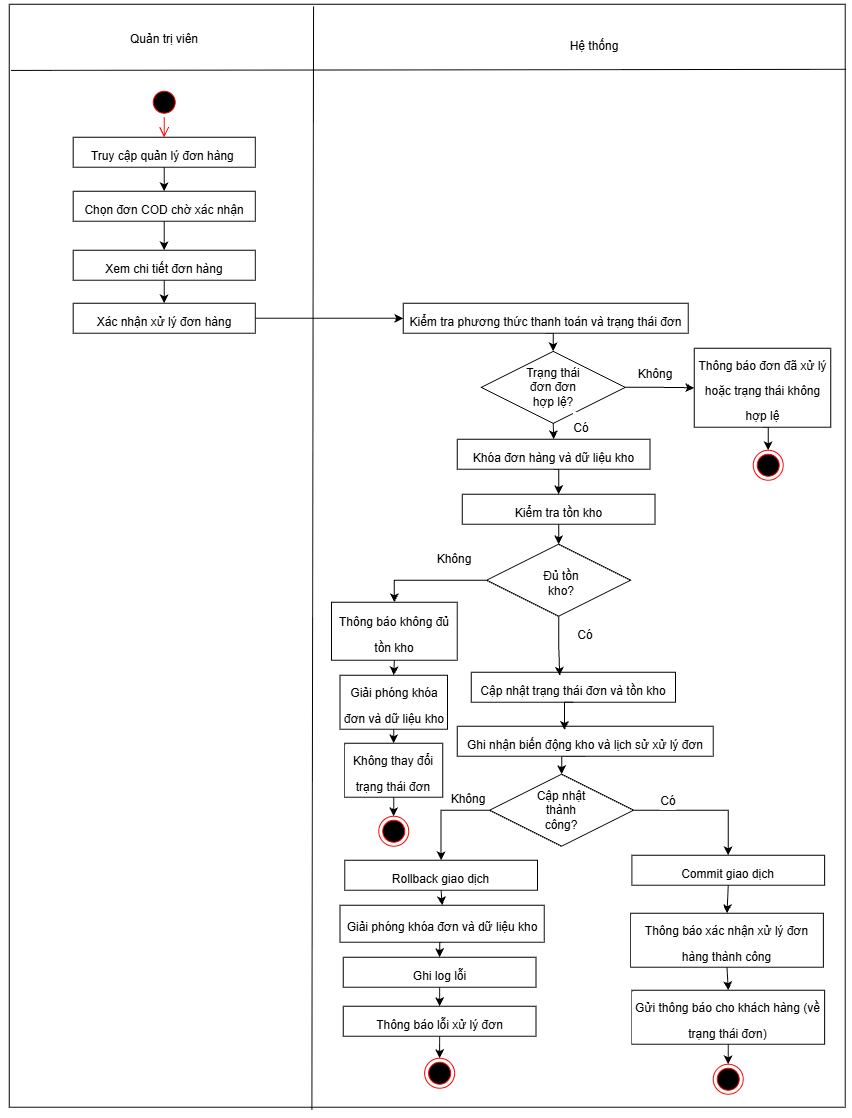
\includegraphics[width=0.94\textwidth,height=0.58\textheight,keepaspectratio]{Images/Activity/da-Xử lý và xác nhận đơn COD.drawio.png}
    \captionof{figure}{Sơ đồ hoạt động xử lý và xác nhận đơn COD}
    \label{appendix:fig:activity-cod-confirmation}
\end{minipage}
\par\medskip

\par\medskip\noindent
\begin{minipage}{\textwidth}
\subsubsection{Đồng bộ chỉ mục AI}

Quản trị viên khởi tạo tác vụ đồng bộ; Backend lấy dữ liệu sản phẩm từ MySQL và
AI Service cập nhật vector trong Qdrant theo từng lô. Sản phẩm lỗi được ghi nhận
để thử lại mà không làm dừng toàn bộ tác vụ.

\centering
    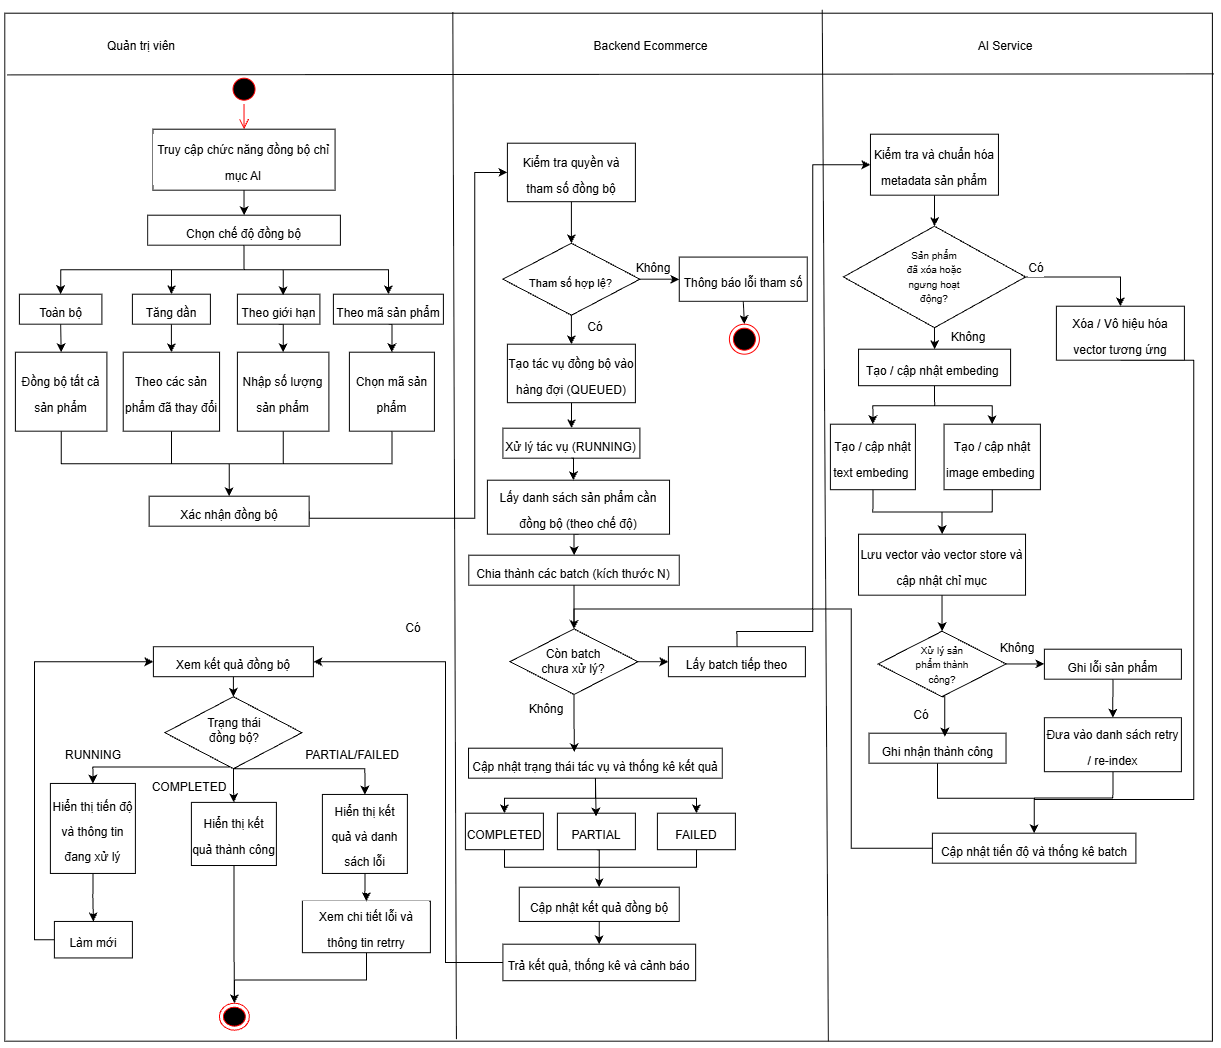
\includegraphics[width=0.94\textwidth,height=0.58\textheight,keepaspectratio]{Images/Activity/da-Đồng bộ chỉ mục AI.drawio.png}
    \captionof{figure}{Sơ đồ hoạt động đồng bộ chỉ mục AI}
    \label{appendix:fig:activity-ai-index-sync}
\end{minipage}
\par\medskip

\FloatBarrier
